\section{Standard Basis}
Standard basis vectors are also known as standard {\bf unit vectors}. These are used to represent vectors in $\mathbb{E}^3$

\begin{definition}
  The standard basis vectors are defined as follows:
  \begin{align*}
    \hat{i} &= (1, 0, 0 ) \\
    \hat{j} &=  (0, 1, 0) \\
    \hat{k} &=  (0, 0, 1)
  \end{align*}
such that $\mid \hat{i} \mid = \mid \hat{j} \mid = \mid \hat{k} \mid.$ 
\end{definition}

Any vector can be represented using standard basis vectors. 

Suppose you are a given a vector $\vec{v} = (v_1, v_2, v_3)$. This can be represented as follows:
\begin{equation}
  \vec{v} = \begin{bmatrix} v_1 \\ v_2 \\ v_3 \end{bmatrix}  =v_1\hat{i} + v_2\hat{j} + v_3\hat{k}
\end{equation}

\begin{eg}
  Let $\vec{v} = (2, 3, 4)$. Then, 
  \begin{align*}
    \vec{v} &= 2\hat{i} + 3\hat{j} + 4\hat{k} \\
    &= 2(1, 0, 0) + 3(0, 1, 0) + 4(0, 0, 1) \\
    &= (2, 0, 0) + (0, 3, 0) + (0, 0, 4) \\
    &= (2, 3, 4)
  \end{align*}
\end{eg}


\begin{figure}[H]
\centering
   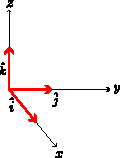
\includegraphics[scale=2.5]{standard-basis.pdf}
   \caption{Standard Basis Vectors}
   \label{fig:figure-3-unit-vector}
\end{figure}

\subsubsection{Algebra with Standard Basis Vectors}
\vspace{5px}
\begin{eg}
  Let $\vec{v}$ and $\vec{w} \in \mathbb{E}^3$ 
  \begin{flalign*}
    \vec{v} \pm \vec{w} = \begin{bmatrix} v_1 \pm w_1 \\ v_2 \pm w_2 \\ v_3 \pm w_3\end{bmatrix}  = (v_1 \pm w_1)\hat{i} + (v_2 \pm w_2)\hat{j} + (v_3 \pm w_3)\hat{k} &
  \end{flalign*}
\end{eg}


\begin{eg}
  Let $\vec{v}$ and $\vec{w} \in \mathbb{E}^3$ 
  \begin{flalign*}
    \lambda\vec{v} = \begin{bmatrix} \lambda v_1 \\ \lambda v_2 \\ \lambda v_3\end{bmatrix}  = (\lambda v_1)\hat{i} + (\lambda v_2)\hat{j} + (\lambda v_3)\hat{k} &
  \end{flalign*}
\end{eg}

\begin{note}
 The 0 vector is:
  $$\underline{0} = \begin{bmatrix} 0 \\ 0 \\ 0 \end{bmatrix} = 0\hat{i} + 0\hat{j} + 0\hat{k}$$
Any vector $\vec{v} \in \mathbb{E}^3$ added to the 0 vector is itself:
$$\vec{v} + \underline{0} = \vec{v}$$
\end{note}

Here is an example of algebra with standard basis vectors:
\begin{eg}
  Let $\vec{v} = (2, 3, 4)$ and $\vec{w} = (1, 2, 3)$. Then,
  \begin{align*}
    \vec{v} + \vec{w} &= (2, 3, 4) + (1, 2, 3) \\
    &= (2 + 1, 3 + 2, 4 + 3) \\
    &= (3, 5, 7)
  \end{align*}
\end{eg}

\subsubsection{Alternate Notation for Standard Basis Vectors}
\vspace{5px}
\begin{notation}
  We can change notation for standard basis vectors as follows:
  $$\hat{i} = \vec{e}_{1} \ \ \ \ \ \ \ \ \hat{j} = \vec{e}_{2} \ \ \ \ \ \ \ \ \hat{k} = \vec{e}_{3}$$
\end{notation}
and therefore we can write:
$$\vec{v} = v_1\hat{i} + v_2\hat{j} + v_3\hat{k} = \sum^{3}_{a=1}v_a \vec{e}_a$$
